% Adapted from http://www.texample.net/tikz/examples/decision-tree/
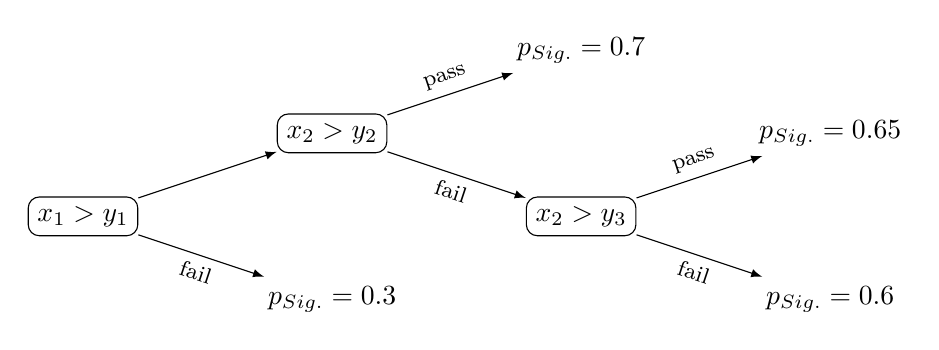
\begin{tikzpicture}
  [
    grow                    = right,
    sibling distance        = 6em,
    level distance          = 9em,
    edge from parent/.style = {draw, -latex,font=\footnotesize},
    sloped,
    treenode/.style = {shape=rectangle, rounded corners,
      draw, align=center},
    root/.style     = {treenode},
    env/.style      = {treenode},
    leaf/.style      = {treenode, draw=white}
  ]
  \node [root] {$x_{1} > y_{1}$}
    child { node [leaf] {$p_{\text{Sig.}} = 0.3$}
      edge from parent node [below] {fail} }
    child { node [env] {$x_{2} > y_{2}$}
      child { node [env] {$x_{2} > y_{3}$}
        child { node [leaf] {$p_{\text{Sig.}} = 0.6$}
          edge from parent node [below] {fail} }
        child { node [leaf] {$p_{\text{Sig.}} = 0.65$}
          edge from parent node [above] {pass} }
        edge from parent node [below] {fail} }
      child { node [leaf] {$p_{\text{Sig.}} = 0.7$}
        edge from parent node [above, align=center]
        {pass} }
    };
\end{tikzpicture}
